\documentclass[a4paper]{article}

\usepackage[margin=0.7in]{geometry}
\usepackage[english]{babel}
\usepackage[utf8]{inputenc}
\usepackage{amsmath}
\usepackage{pxfonts}
\usepackage{graphicx}
\usepackage[colorinlistoftodos]{todonotes}
\usepackage{listings,fontspec}
\usepackage{float}
\usepackage{upgreek}
\usepackage{ amssymb }
\usepackage{titling}
\usepackage{wrapfig}

\setlength{\droptitle}{-9em}

\lstset{
  basicstyle=\small\ttfamily,
  language= R,
  frame=single,
  numbers=none,
  showstringspaces=false
}
\lstloadlanguages{R}
\lstset{escapeinside={(*@}{@*)}}


\title{Homework 5}

\author{Gitanshu Munjal}

\date{November 14, 2014}

\begin{document}
\maketitle

\section{Principal Component Analysis}

\subsection{}Perform a PCA on the 14 soil variables (do not include biomass) using the correlation matrix. [5]


\subsubsection{Code and Relevant Output}
\begin{lstlisting}[language=R]
install.packages(c("corrplot","psych", "caret","mvnormtest"))

library(mvnormtest)
library(psych)
library(corrplot)
library(caret)

spartina<-read.csv("C:\\Users\\gitanshu\\Desktop\\spartina.txt", header=T)
spa<-spartina[,4:17]

spa.pca<-princomp(spa[,1:14], data=spa, cor=TRUE, scores=TRUE)
summary(spa.pca)
\end{lstlisting}


\begin{lstlisting}[language=R,frame=none]
Importance of components:
                          Comp.1    Comp.2    Comp.3     Comp.4     Comp.5     Comp.6
Standard deviation     2.2189883 1.9222969 1.2677248 1.15537939 0.83162354 0.70750645
Proportion of Variance 0.3517078 0.2639447 0.1147947 0.09535011 0.04939984 0.03575467
Cumulative Proportion  0.3517078 0.6156525 0.7304472 0.82579732 0.87519715 0.91095182
                           Comp.7     Comp.8     Comp.9    Comp.10     Comp.11     Comp.12
Standard deviation     0.62083663 0.61706787 0.40739295 0.37814467 0.294731964 0.212812256
Proportion of Variance 0.02753129 0.02719805 0.01185493 0.01021381 0.006204781 0.003234933
Cumulative Proportion  0.93848312 0.96568117 0.97753610 0.98774991 0.993954695 0.997189627
                           Comp.13      Comp.14
Standard deviation     0.172779077 0.0974300126
Proportion of Variance 0.002132329 0.0006780434
Cumulative Proportion  0.999321957 1.0000000000
\end{lstlisting}
\begin{center}
\line(1,0){250}
\end{center}




\subsection{} How many PC�s are found? Explain why. [10] \\
\\\textbf{14 PC's are found because the PCA is appled to 14 variables} (the explanatory variables in our original data). The model concept of PCA uses the number of variables (say n) specified by the data to calculate linear combinations of variables to produce n orthongonal principal components.
\begin{center}
\line(1,0){250}
\end{center}
\pagebreak



\subsection{}What is the numerical value of the eigenvalue for PC7? [5]
\subsubsection{Code And Relevant Output}
\begin{lstlisting}[language=R]
(summary(spa.pca)$sdev[7])^2           #numerical value of the eigenvalue for PC7
\end{lstlisting}

\begin{lstlisting}[language=R,frame=none]
   Comp.7 
(*@\textcolor{blue}{0.3854381}@*) 
\end{lstlisting}

\begin{lstlisting}[language=R]
correlations<-cor(spa)
eigen(correlations)$values[7]          #numerical value of the eigenvalue for PC7
\end{lstlisting}


\begin{lstlisting}[language=R,frame=none]
[1] (*@\textcolor{blue}{0.3854381}@*)
\end{lstlisting}
\begin{center}
\line(1,0){250}
\end{center}



\subsection{}What is the sum of the eigenvalues? Why? [5]
\subsubsection{Code And Relevant Output}
\begin{lstlisting}[language=R]
sum((summary(spa.pca)$sdev)^2)         #sum of eigenvalues
\end{lstlisting}
\begin{lstlisting}[language=R,frame=none]
[1] (*@\textcolor{blue}{14}@*)
\end{lstlisting}

\begin{lstlisting}[language=R]
sum(eigen(correlations)$values)        #sum of eigenvalues
\end{lstlisting}
\begin{lstlisting}[language=R,frame=none]
[1] (*@\textcolor{blue}{14}@*)
\end{lstlisting}

Our current PCA model uses the correlation matrix (see 1.1). We know that a correlation matrix  is the equivalent to a covriance matrix of the standardized variables. We also know that standardized variables have a mean of 0 and a variance of 1. We also know that the total variance of our PCA (sum of eigenvalues) is equal to the total variance of our model. \textbf{Conclusively, the sum of eigenvalues (total variance of PCA) should be equal to the number of original variables as each variable contributes a variance of 1 (because it is standardized as mentioned earlier) towards the total variance.}
\begin{center}
\line(1,0){250}
\end{center}



\subsection{}What proportion of the variation or information of the original data set would be retained if you only keep 2 PC's? How many PC�s would you retain? Why? [10]
\subsubsection{Code And Relevant Output}
\begin{lstlisting}[language=R]
keep2 <- sum((summary(spa.pca)$sdev[1:2])^2)
totalvariance <- sum((summary(spa.pca)$sdev)^2)
keep2proportion <- keep2/totalvariance
keep2proportion                        #What proportion of the variation...
\end{lstlisting}
\begin{lstlisting}[language=R,frame=none]
[1] (*@\textcolor{blue}{0.6156525}@*)
\end{lstlisting}
61.6\% proportion of the variation or information of the original data set would be retained if we only kept the first 2 PC's. It is advisable to \textbf{retain enough Principal Components to account for a critical amount (80\% here subjectively) of the total variance of the original data} and so according to that definition we should retain the \textbf{first 4 PC's} here (Cumulative Proportion 82.58\%, see 1.1).
\begin{center}
\line(1,0){250}
\end{center}


\subsection{}Make a scatterplot of the scores on PC2 vs. scores on PC1, and describe any patterns detected. [5]
\subsubsection{Code and Relevant Output}
\begin{lstlisting}[language=R]
pc1scores <- spa.pca$scores[,1]
pc2scores <- spa.pca$scores[,2]
plot(pc1scores,pc2scores, xlab="PC1 scores", ylab="PC2 scores", pch=21)
\end{lstlisting}

\begin{figure}[H]
\centering
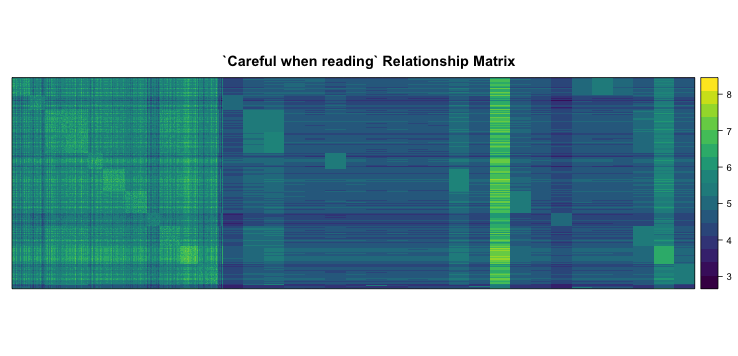
\includegraphics[width=0.6\textwidth]{Rplot.jpeg}\\
\caption{\label{fig:Rplot} scatterplot of the scores on PC2 vs. scores on PC1}
\end{figure}
The above scatterplot has a possible directly proportional (linear) pattern between the 2 PC's but outliers to this pattern are easily seen.
\begin{center}
\line(1,0){250}
\end{center}


\subsection{}Make a biplot and interpret it. Are there "synthetic" dimensions? How do they make sense in terms of soil properties? [10]
\subsubsection{Code And Relevant Output}
\begin{lstlisting}[language=R]
biplot(spa.pca)
\end{lstlisting}
\begin{figure}[H]
\centering
\includegraphics[width=0.6\textwidth]{Rplot01.jpeg}\\
\caption{\label{fig:Rplot01} Gabriel's biplot}
\end{figure}
The above biplot shows two bundles of variables (synthetic dimensions); one dominantly across PC1  (pH, Ca,NH4,acid,Zn,P)and the other dominantly across PC2(K,Na,Mg). These dimensions present signatures of possible pH gradient like and CEC activity. Soil acidity and alkalinity are known to be one of the most significant soil properties and so the appearance of such a gradient across PC1 (most variance explained) should not be a surprise. 


\section{Bootstrapping}
\subsection{}Use bootstrapping to make a 95\% confidence interval for the first eigenvalue in the spartina soil data.Report your code. [10]
\subsubsection{Code}
\begin{lstlisting}[language=R]
install.packages("boot")
library(boot)

pca4boot <- function(data, i) {
  data.i <- data[i,]
  pca.i <- prcomp(data.i[,4:17], scale.=T)
  eval1 <- pca.i$sdev[1]^2
  return(eval1)
}

boot.results <- boot(spartina,pca4boot,1999)
boot.ci(boot.results)
\end{lstlisting}
\begin{center}
\line(1,0){250}
\end{center}


\subsection{}What are the bca CI and the bias for the first eigenvalue? [10]
\subsubsection{Code And Relevant Output}
\begin{lstlisting}[language=R]
boot.ci(boot.results)
\end{lstlisting}
\begin{lstlisting}[language=R,frame=none]
CALL : 
boot.ci(boot.out = boot.results)

Intervals : 
Level      Normal              Basic         
95%   ( 3.823,  5.419 )   ( 3.779,  5.363 )  

Level     Percentile            (*@\textcolor{blue}{BCa}@*)          
95%   ( 4.485,  6.069 )   (*@\textcolor{blue}{( 3.853,  5.429 )}@*)  
Calculations and Intervals on Original Scale
Warning : BCa Intervals used Extreme Quantiles
Some BCa intervals may be unstable
\end{lstlisting}

\begin{lstlisting}[language=R]
boot.results
\end{lstlisting}
\begin{lstlisting}[language=R,frame=none]
ORDINARY NONPARAMETRIC BOOTSTRAP


Call:
boot(data = spartina, statistic = pca4boot, R = 1999)


Bootstrap Statistics :
    original   (*@\textcolor{blue}{bias}@*)    std. error
t1* 4.923909 (*@\textcolor{blue}{0.302691}@*)   0.4070658
\end{lstlisting}
\begin{center}
\line(1,0){250}
\end{center}
\pagebreak

\subsection{}Is the first eigenvalue significantly different from 1? [5]
\subsubsection{Code And Relevant Output}
\begin{lstlisting}[language=R]
firsteig<-vector()
firsteig<-boot.results[2]
firsteig<-unlist(firsteig)
t.test(firsteig,conf.level=0.95,mu=1)
\end{lstlisting}

\begin{lstlisting}[language=R,frame=none]
	One Sample t-test

data:  firsteig
t = 464.2297, df = 1998, (*@\textcolor{blue}{p-value < 2.2e-16}@*)
alternative hypothesis: true mean is not equal to 1
95 percent confidence interval:
 5.208745 5.244456
sample estimates:
mean of x 
   5.2266 
\end{lstlisting}
Exclusion of 1 from the most liberal (and biased) \textbf{confidence intervals earlier generated in section 2.2} and the significant p-value for the above presented \textbf{two tailed t-test both indicate that indeed the first eigenvalue is significantly differnt from 1}.
\begin{center}
\line(1,0){250}
\end{center}


\subsection{}What are the main types of bootstrapping in multiple linear regression and how would you determine which one to apply? [10]\linebreak
\linebreak Case resampling and residual resampling are the the two main types of bootstrapping in MLR. The first kind (case resampling) is used in conditions or where there is uncertainty about the proposed model or we suspect violation of assumptions about the residual variance or if predictor values are not fixed (random X). \textbf{Under case resampling whole observations (cases) are resampled when bootstrapping}. The second kind (residual resampling) is used in happy conditions where we know our model to be good, variances to be homogeneous, and predictors to be fixed in value (fixed X). \textbf{Under residual resampling, residuals are resampled (and added to predicted values) and are used for bootstrapping}.
\begin{center}
\line(1,0){250}
\end{center}

\subsection{}What are the two key arguments that must appear in the function to be called from inside the boot() function? [5] \linebreak
\linebreak Data ("data" in our case) and  a vector of indices, frequencies or weights which define the bootstrap sample ("i" in our case) are the two key arguments that must appear in the function to be called from inside the boot() function.
\begin{center}
\line(1,0){250}
\end{center}
\pagebreak

\subsection{}How is the percentile CI calculated in bootCI()? [10]\\ 
\linebreak 
The percentile CI is calculated in bootCI based on quantiles (using two-sided probabilities for the confidence level) obtained from the histogram of estimated partial regression coefficients.\\
\subsubsection{Code And Relevant Output}
\begin{lstlisting}[language=R]
boot.ci(boot.results)
\end{lstlisting}
\begin{lstlisting}[language=R,frame=none]
CALL : 
boot.ci(boot.out = boot.results)

Intervals : 
Level      Normal              Basic         
95%   ( 3.823,  5.419 )   ( 3.779,  5.363 )  

Level     (*@\textcolor{blue}{Percentile}@*)            BCa          
95%   (*@\textcolor{blue}{( 4.485,  6.069 )}@*)     ( 3.853,  5.429 )
Calculations and Intervals on Original Scale
Warning : BCa Intervals used Extreme Quantiles
Some BCa intervals may be unstable
\end{lstlisting}
\begin{lstlisting}[language=R]
firsteig<-vector()
firsteig<-boot.results[2]
firsteig<-unlist(firsteig)
quantile(firsteig,probs=c(0.025,0.975))
\end{lstlisting}
\begin{lstlisting}[language=R,frame=none]
    2.5%    97.5% 
4.485456 6.078309 
\end{lstlisting}
\begin{center}
\line(1,0){250}
\end{center}
\end{document}

